\documentclass[conference]{IEEEtran}
% The preceding line is only needed to identify funding in the first footnote. If that is unneeded, please comment it out.
\usepackage{url,apacite}
\usepackage{amsmath,amssymb,amsfonts}
\usepackage{algorithmic}
\usepackage{graphicx}
\usepackage{textcomp}
\usepackage{xcolor}
\usepackage{natbib}
\graphicspath{ {.} }
\bibliographystyle{apacite}
\def\BibTeX{{\rm B\kern-.05em{\sc i\kern-.025em b}\kern-.08em
T\kern-.1667em\lower.7ex\hbox{E}\kern-.125emX}}

\usepackage{listings}
\usepackage{xcolor}
 
\definecolor{codegreen}{rgb}{0,0.6,0}
\definecolor{codegray}{rgb}{0.5,0.5,0.5}
\definecolor{codepurple}{rgb}{0.58,0,0.82}
\definecolor{backcolour}{rgb}{0.95,0.95,0.92}

\lstdefinestyle{mystyle}{
    backgroundcolor=\color{backcolour},   
    commentstyle=\color{codegreen},
    keywordstyle=\color{magenta},
    numberstyle=\tiny\color{codegray},
    stringstyle=\color{codepurple},
    basicstyle=\ttfamily\footnotesize,
    breakatwhitespace=false,         
    breaklines=true,                 
    captionpos=b,                    
    keepspaces=true,                 
    numbers=left,                    
    numbersep=5pt,                  
    showspaces=false,                
    showstringspaces=false,
    showtabs=false,                  
    tabsize=2
}
     
\lstset{style=mystyle}

\begin{document}

\title{A microservices based approach for city traffic simulation}

\author{\IEEEauthorblockN{1\textsuperscript{st} Toma Becea}
    \IEEEauthorblockA{\textit{Automation and Computer Science Faculty} \\
    \textit{Technical University of Cluj-Napoca}\\
            Cluj-Napoca, Romania \\
            tomabecea@pm.me}
    \and
    \IEEEauthorblockN{2\textsuperscript{nd} Honoriu V{\~a}lean}
    \IEEEauthorblockA{\textit{Automation and Computer Science Faculty} \\
    \textit{Technical University of Cluj-Napoca}\\
            Cluj-Napoca, Romania \\
            Honoriu.Valean@aut.utcluj.ro}
}

\maketitle

\begin{abstract}

Simulating traffic in a city is a difficult task. Current paper is proposing a novel way using state of the art in distributed systems: microservices orchestration. The design is centered around two types of actors: a city simulation actor (a single instance of it) which keeps track of occupied streets and and their gradual occupation. The other actor type (multiple instances) is the car which travels across the city.

\end{abstract}

\section{Introduction}

A solution which simulates car, pedestrian, etc. traffic in a given city may reap many benefits. It can help understand patterns of traffic and its flow. It can help unerstand the particularities and pecularities of a city's streets arrangements. It can help identify bottlenecks. It can help find solutions to rush problems and explore them. But for those areas to be tackled, appropiate methods of simulating traffic must be found. We are proposing a novel way of simulating traffic based on the microservices orchestration concept.

We define a \textbf{(city) actor} as being a independent entity which chose to move between two geographical points within a city. It can be a car, a pedestrian or a bike. We also define the \textbf{city simulator} as being a single entity (subject to distributed and load balacing services) which keeps data about the city (e.g. streets with city actors on them).

This paper is structured in few sections. Section \ref{sec:existingsolutions} contains a summary of few other papers and ideas around the same subject of traffic simulatino. Section \ref{sec:implementation} discuss the core approach of the current paper in architecting a software solution based on microservices for simulating traffic in a city. Section \ref{sec:orchestration} discuss the architectural aspect of orchestrating microservices using popular frameworks and solutions. Section \ref{sec:results} presents the results obtained after the implementation of some of the core concepts from the previous sections.

\section{Existing solutions}
\label{sec:existingsolutions}

(Summary of other papers with traffic simulation)

\section{Implementation}
\label{sec:implementation}

The entities which are participating into a traffic simulation are called actors. They are two: the city actor and the city simulator. The supporting containers are not themselves part of traffic simulation but they do have an important and supporting role. All of them are modeled as microservices and a short introductory is needed altought section \ref{sec:orchestration} and paragraph \ref{subsec:designchoices} offers a broader perspective around them.

\subsection{Microservices}

Microservices are not a new concept. The idea behind them has existed since Linux kernel has started to be enriched with a concept called namespaces \citep{wiki:linuxns}. This allows one set of processes to see one set of resources while another set of processes see another set of resources, where resources might be, but not limited to, process IDs, file names and network resources. Those linux kernel abilities form the base of containers.

Thus, a container is a small set of processes which run in isolation. They allow packaging a linux distro, a set of libraries and skd and on top of those custom code. This forms an image, which is essentially a tar gzipped file. Once the build process of an image is finished, it can be spinned up in one or more running containers. The custom code written and embedded in the image is running in parallel in each container.

To go to solution for building, manipulating and running images is Docker \citep{docker}. It allows easy software installation, it works cross platform and it offers a smooth experience most of the time.

\subsection{City simulator}

The most common and easy solution to share data across all the city actors is to have a centralized store to keep it. City simulator acts as a centralized store for all other city actors. In the current implementation the city simulator keeps a set of data which can be described as a list of pairs, each pair having a line and a real number, called density.

The density is defined as the number of actors (cars) which are at a given moment present on a given segment of street. If the city simulator has no entry of a street segment then it will consider the density as being 0, i.e. there is no actor on that street. The density is modeled as an unsigned integer.

Figure \ref{fig:citysimrelations} depicts the city simulator in relation with the other entities. A notable exception is the web page. Its purpose is not to participate in the same information exchange the other entities have but to offer a visual interpretation of the way the city and the other actors are interacting with one another.

\begin{figure}
    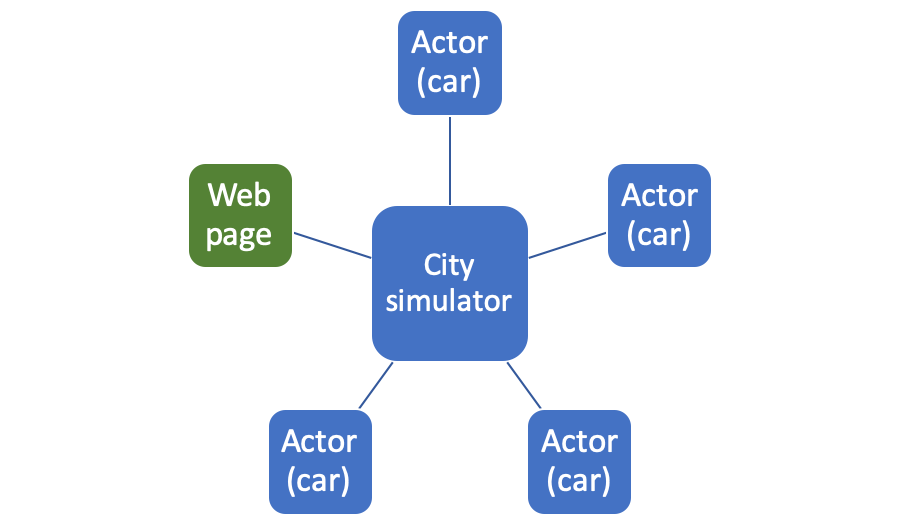
\includegraphics[width=8cm]{CitySimulator.png}
    \centering
    \caption{The relations of city simulator with other entities}
    \label{fig:citysimrelations}
\end{figure}

As various actors send data about their location, the city simulator needs to keep location and density data in its store. It does not know of Open Street Map maps and its corresponding map data sets but instead it requires any actor to send its current set of coordinates which it is crossing or which it left. If any other actor send the same set of coordinates, or a subset of it then the first set of coordinates will have its density incremented. Listing \ref{lst:goactorstruct} shows the Go struct which is used by an actor to send its report to the city simulator and is used by the city simulator to decode a message received from an actor. Apart from this line there are two more details to complete the report picture. Listing \ref{lst:goactorreports} contains the type of communications between actors and the citysimulator.

\begin{lstlisting}[caption=Go struct for actor's report, label=lst:goactorstruct]
// Report is the base type for reporting
// status and vectors to a city entity
type Report struct {
	CurrentLine  [][]float64
	ReportDetail int
}
\end{lstlisting}

As part of this proposal the city simulator is made to be a standalone entity (container) which communicates with actors. This might not be the case for other types of communications, as part of other architectures. One example can be the integration or the unifying of the city simulator with the city actor, both becoming one entity. In this case the communication between entities is subject to an entire panoply of choices.

\subsection{Car actor}

The city actor represents a moving actor within a city. It can be a car which moves across the city, it can be a bike or it can be a pedestrian. Its naming suggests that it can be any entity or living being which moves within a city and interacts with the other entities or affects the other entities in some manner. A pedestrian would directly interact with other pedestrians but not with cars. A pedestrian would indirectly affect other cars by willing to walk over a street crossing.

The implementation proposed here is aiming to model a single type of actor: a car which moves between two points across a city. Because the purpose of this paper is not to tackle maps representation and routing through a city (in itself, this area is way bigger than a mere technical paper) the city actor is using two notable services: Open Street Map \citep{openstreetmap} and GraphHopper \citep{graphhopper}. Open Street Map is an open source licensed map of the entire world. Graphhoper is an open source service which offers directions APIs and route planning. It can use Open Street Map as an underlying map provider. They provider free tiers and paid subscription for accessing an API and get routes. However, a city actor is not using any public api but a special crafted container which contains GraphHopper and an open street map embedded into it. Thus, this container is running in parallel with the other city actors and provides them with the routing API they need.

A first way to introduce randomness into the entire simulation of a city is to choose a set of two coordinates inside the given city, a set for each city actor. Then the actor proceeds to ask GraphHopper service for a route between those two points. Because each city actor 'lives' only while its moving across its route and 'dies' as soon as it reached the finish point, the entire city simulation which takes place is made of independent, random and always new actors.

\subsection{Interactions}

An actor interacts, for the time being, only with the city simulator by using a Go struct and a Go enum. They can be seen in listings \ref{lst:goactorstruct} and \ref{lst:goactorreports}. The message sent from one side to another has a general structure called \textit{Envelope}. It is meant to offer a top level message which can be serialized (or encoded, the way to do this in Golgang, if not gRPC, is the gob pacakge it offers out of the box) and passed around, enabling any party involved to understand what this message is about and how to decode it.

Listing \ref{lst:goenvelope} show the top level message. It contains a message type which instructs the reader what kind of message it has to deal with and the possible types are the second part of listing \ref{lst:goactorstruct}: \textit{SendReport}, \textit{AskForLine}, \textit{RespondWithLine}. Let's take them one by one. \textit{SendReport} represents a message sent from an actor to the city simulator and the \textit{Payload} contains the report seen in listing \ref{lst:goactorreports}. 

\textit{AskForLine} is a message sent from an actor to the city simulator in which the actor asks about the density of any line. This way any actor can take conscious decisions on which route to go on when based on what lies ahead in terms of street densities. When a first route is known, between two desired points, the actor can ask about each line it has on that route. The city simulator will respond with the known density of it. If the actor desires, it can try to find another route by asking GraphHopper service to compute a new one but with an additional rule: avoid a certain point (street, junction, etc.). \textit{RespondWithLine} is the type of message which the city simulator sends back to an actor after it received an \textit{AskForLine} message.

\begin{lstlisting}[caption=Go enumerations for messaging, label=lst:goactorreports]
const (   
    // ReportOnTheLine is the report sent by one agent to
    // notify the city that he is currently advancing
    // through one line.
    ReportOnTheLine = iota
    
    // ReportOffFromLine is the report sent by one agent to
    // notify the city that he has finished advancing through
    // one line and has departed from it.
    ReportOffFromLine = iota
)
    
const (
    // SendReport is a message passed from an actor to the city
    // indicating its status (e.g. location).
    SendReport = iota
    
    // AskForLine is a message passed from an actor to the city.
    // A response is awaited.
    AskForLine = iota
    
    // RespondWithLine is a message passed from the city to
    // an actor and it contains line data.
    RespondWithLine = iota
)
\end{lstlisting}

\begin{lstlisting}[caption=Go top level struct (envelope), label=lst:goenvelope]
// Envelope is the container for different messages sent back
// and forth between an actor and a city
type Envelope struct {
    MessageType int
    Payload     interface{}
}
\end{lstlisting}

\subsection{Design choices}
\label{subsec:designchoices}

As with every software project started from scratch there are a number of choices to make when choosing software stacks, programming languages, networking models, etc. This section is aiming to explore the rationale behind some of those decisions and how they influenced the final application of building such an application.

\begin{itemize}
\item Go programming language
\item Web page choices (web page will become an actor)
\end{itemize}

\subsection{Alternatives}
(Actor model and consacrated frameworks)

\section{Orchestration}
\label{sec:orchestration}

The term orchestration means the handling of containers and microservices in order to bring coherence into their interaction and an unifying experience to the end user of a service or of a product. They migth run on multiple nodes (computers or virtual machines) and at the same time they need to communicate with one another. They need to be updated in place and without service disruption. Whenever one of them crash they have to restart as quickly as possible. They have to be able to discover themselves without dealing with intricancies of IP addresses, proxies, etc. Those are just few concerns around orchestration and the current paper is not aiming to provide a comprehensive view of what it means and what can be achieved with it but rather to set a basis of understanding enough context for the subject of simulating a city with its traffic.

\cite{7922500} offers a comprehensive view of the current state of orchestration of cloud providers. (to add details)

\subsection{Current state}

As noted above the standard in easiness of developing and working with containers is Docker \citep{docker}. While it has an offering of orchestrating containers, called \textit{docker-compose}, which is simple to start with, its functionality is limited in comparison with other offerings, the most notable one being Kubernetes \citep{Kubernetes}. Those are not the single tools available and many more can be found but they offer a starting point (especially Docker) and Kubernetes, altough it has a steep learning curve, it does offer a comprehensive and complex panoply of details around orchestration.


\subsection{Implementation}

The city simulator is, currently, a single service which means it runs as a single instance. The city actor container runs in multiple instances and it has the need to do so as part of the entire simulation workload. The other two instances which run in the simulation are the routing service, a Graphhopper instance, and the front end web erver which displays a web page for offering visual clues around the simulation. While they run as such there should be an easy way, without friction and additional compute logic to "discover" a certain service. A city actor will need to create connect itself to the routing service and to the city simulator. At the same time the front end instance need to connect itself to the city simulator to source its data.

\subsection{Docker compose}

The \textit{docker-compose} tool gives the ability to manipulate more containers and services, with a simple file written in yaml format. Listing \ref{lst:dockercompose} shows the docker-compose file in its brevity and briefness. Let's dissect it. There are four services: \textit{graphhopper}, \textit{citysim}, \textit{cityactor} and \textit{cityfront}. Each of them need an image to run and this image can be specified in two ways: either as an image already compiled and hosted on an container registry or as a local folder which contains an file to build one (defined by the presence of a file called \textit{dockerfile}). Because Graphhoper, once compiled with desired maps and settings do not need any more development work, it is taken as an image from a docker registry. The other three services are the places where the most development efforts take place therefore they need to be compiled or recompiled each time the entire traffic simulation application starts.

The containers which are running may need to have different properties. First and most important is the container port which needs to be published. The port from inside the container, where a certain process expect a TCP communication is forwarded to the local host port and thus is accessible from outside the Docker internal network. Another detail of the container is its dependency. For example \textit{cityactor} cannot run without textit{Graphhopper} because it doesn't have any place to obtain a route. Therefore it depends on \textit{Graphhopper}. And on \textit{citysim}, of course. The last bit of detail which can be seen here is the policy of restarting a container. By default the policy is set to "No" which means that the container will not be restarted if there is any failure within it and it stops. However, for simulation purposes, as we need a constant stream of city actors to swarm through the city, the policy is set to "Always" which will restart the container after if closes itself, i.e. it finishes its travel.

\begin{lstlisting}[caption=Docker-compose file, label=lst:dockercompose]
services:
  graphhopper:
    image: tomabecea/graphhopper:latest
    ports:
      - "8989:8989"
  citysim:
    build: ./city/citysim
    ports:
      - "9000:9000"
  cityactor:
    build: ./city/cityactor
    depends_on: 
      - "graphhopper"
    restart: always
  cityfront:
    build: ./cityfront
    ports:
      - "80:80"
    depends_on:
      - "citysim"
\end{lstlisting}

Finally, to run this docker compose there is a simple command to bring everything to life: \textit{\textbf{docker-compose up}}. This will take everything which is in the \textit{docker-compose.yaml} file, will build the container if it has not been built before or if any source code file has been changed and then will run all of them in the order specified by the dependency graph.

The other detail of running this set of containers is to scale up a specific service. In our case we would like to have more than one city actor. Therefore the command to run is \textit{\textbf{docker-compose up --scale cityactor=1001}}. This way one thousand and one city actors will be created. In combination with the option of always restarting a container which exits, the entire simulation will run virtually forever.

\subsection{Kubernetes}

While the docker compose offers a basic set of functionalities to bootstrap our application, for a large number of city actors a single computer might not suffice. Here comes Kubernetes in play. Kubernetes \citep{Kubernetes} is an open-source system for automating deployment, scaling and management of containerized applications. It originates from Google and is their third approach on orchestrating microservices, as described in \cite{burns2016borg}.

While Docker-Compose runs on a single machine, Kubernetes is made to run on multiple machines called nodes. It is by default enriched with certain abilities needed to run in this configuration. Made initially to run with LXC and Docker containers \citep{7036275}, it is now a more open system where one can choose the container runtime interface, the container network interface, storage interface, service meshes, etc. from a broad range of vendors. On top of those base offerings, which provides only the backbone of Kubernetes, a distributed application must be built. The desired architecture of a Kubernetes application may consists of many concepts and building bricks. Using \cite{hightower2017kubernetes} as a starting point we can see that there are the most simple and basic units, called pods, which may encompass one or more containers (usually there is one main container and the others, e.g. service mesh supporting side car, are called side cars). There are deployments which gather together pods and rollout or rollback control. There are services which makes pods universally available into the cluster and makes them discoverable, regardless of what node are they running onto and abstracting away failures and upgrades. And then there are replica sets, daemon sets, secrets, config maps and many other resources. On top of those one is able to deploy own custom resource definitions as well as custom controllers. Put together, all those concepts have a rather intimdating allure.

For running the entire traffic simulation onto a Kubernetes cluster we have the basic needs: all services are Docker images. Once each service is correctly described using a yaml format, each consisting of a service and deployment the entire application can be deployed via \textit{kubectl} command. The scaling problem is solved using a similar approach with \textit{docker-compose}. The command will be \textit{\textbf{kubectl scale --replicas=1001 deployment/cityactor}}. As before, with \textit{docker-compose}, it is to be noted the simple approach towards scaling: a core tenet of distributed systems, a property which, as it stands for our use case is quite simple to model. But for other applications, a more sensible approach is needed, as noted by \cite{jogalekar2000evaluating}.

\subsection{Networking design}
\label{subsec:networking}

A distributed system has to carefully design the way in which its services communicates between them. As the nature of a distributed system is to run in multiple nodes or machines, it is obvious that the communication medium between them has to be one based on TCP/IP stack. Therefore the entire modeling of networking relies on this assumption.

A simple and basic idea, noted here only to help on constructing the final proposed solution, is to have each service always located at a certain IP address and a certain port within a network. This means, for example, the city simulator will always be located at 192.168.0.101:7450. The other services which need to be accessed will listen on similar IP addresses and sockets. While this offers a convenient way to have them unified, they are not suitable to run in other environments than a development PC. In this case \textit{docker-compse} will run them such that they are accessible on local host address, i.e. 127.0.0.1:7450. As soon as there are multiple nodes involved this model is not suitable anymore.

Enter the DNS (Domain Name System), the backbone of the entire internet. In its simplest description, avoiding many inherent and nitpicking details, it is a dictionary which keeps track of every registered and easy to memorize name, e.g. en.wikipedia.com and the IP addresses where it is located. Any client which would like to access such an name will query first the DNS resolvers and then it will proceed to send a message to the obtain IP address. The most notable interaction of a user with the DNS is the address bar of a browser where the user inserts the name of the site they want to access and while writing the address suggestions are displayed by the browser with the help of recommandation engines \citep{risley2001domain}.

When many resources are needed, to serve a great number of users or to support a great number of city actors, a certain service might be so busy with serving data that the compute and memory resources it needs are greater than the hardware is able to give. Therefore it might be located at few addresses at the same time and any client which wants to access it should access the address where there are available compute and memory resources to serve its queries. Ideal would be to abstract or to decouple this information from the client and make it transparent for it. To do this the client needs to know only the service name and a certain "networking" entity should route its request to the appropiate available service. Such a entity could be a DNS authoritative server which, based on the load, availability and latency of the services will route the request to the appropiate node \citep{swildens2006scalable}.

Docker and Kubernetes are doing a similar job. They offer a DNS service and according to the load of each node where a service run, a request is rooted to a node which will be able to respond to it. This logic is completely decoupled from the clients. Listings \ref{lst:gocityclientdial} and \ref{lst:cityfrontclientdial} shows how both the city front and a city actor calls the city simulator. All what they do is to use the address which was specified in the docker-compose file (listing \ref{lst:dockercompose}). Docker or Kubernetes will do the actual job to route the request to the appropiate node of the service.

\begin{lstlisting}[caption=City client dialing City simulator, label=lst:gocityclientdial]
conn, err := net.Dial("tcp", "citysim:7450")
if err != nil {
    fmt.Println("Error on dialing", err)
    break
}
defer conn.Close()
\end{lstlisting}

\begin{lstlisting}[caption=City front dialing City simulator, label=lst:cityfrontclientdial]
var startWebsocket = function (callback) {

    var ws = new WebSocket("ws://citysim:9000/city")

    ws.onopen = function(evt) {
        console.log("OPEN");
        ws.send("just sent some messageeeee")
    }
    ws.onclose = function(evt) {
        console.log("CLOSE");
        ws = null;
    }
    ws.onmessage = function(evt) {
        callback(evt.data);
    }
    ws.onerror = function(evt) {
        console.log("ERROR: " + evt.data);
    }
}
\end{lstlisting}

\section{Results}
\label{sec:results}

\subsection{Visual}

\subsection{Performance}

\section{Enhancements}
\label{sec:enhancements}
(Distributed database for multiple city simulators)

(More granular logic on actor behavior)

(More types of "junctions": classic junction for cars, pedestrian crossings, subways access stairs and elevators, bus stations, etc.)

(Contained actors: pedestrians in a bus, pedestrian in a subway)

\bibliography{wiki}
\vspace{12pt}

\end{document}
